\documentclass[aps,prb,superscriptaddress,nofootinbib]{revtex4}
\usepackage{amsfonts}
\usepackage{amsmath}
\usepackage{amssymb}
\usepackage{graphbox}
\usepackage{graphicx}
\usepackage{caption}
\usepackage{bm}
\usepackage{bbm}
\usepackage{cancel}
\usepackage{color}
\usepackage{mathrsfs}
\usepackage[colorlinks,bookmarks=true,citecolor=blue,linkcolor=red,urlcolor=blue]{hyperref}
\usepackage{simpler-wick}
\usepackage{appendix}
\usepackage{float}
\usepackage{array}
\usepackage{booktabs}
\usepackage[export]{adjustbox}
\setlength{\parindent}{10 pt}
\setlength{\parskip}{2 pt}
\setcounter{MaxMatrixCols}{30}
\bibliographystyle{apsrev}
\newcommand{\RNum}[1]{\uppercase\expandafter{\romannumeral #1\relax}}
\newcommand{\normord}[1]{{:\mathrel{#1}:}}
\def\tbs{\textbackslash}
\def \tr{\operatorname{tr}}
\def \Tr{\operatorname{Tr}}


\begin{document}
\title{Nonlinear Sigma Model}
\author{Jie Ren}


\maketitle

In the context of spontaneous breaking of continuous symmetries, the nonlinear sigma model (NL$\sigma$M) arises as the effective description of the low energy physics.

\tableofcontents

\section{Field Theory of Lie Groups}

\subsection{NL$\sigma$M for U(1) Group}
Consider the complex $\phi^4$ theory with negative mass term:
\begin{equation}
	\mathcal L = \partial^\mu \phi^* \partial_\mu \phi + m^2\phi^* \phi - \frac{g}{4}(\phi^*\phi)^2.
\end{equation}
The minimal energy field configuration is $|\phi_0|^2 = 2m^2/g$.
The field can be parameterized as
\begin{equation}
	\phi(x)=\left[\sqrt{\frac{2 m^{2}}{g}}+\frac{\sigma(x)}{\sqrt{2}} \right] \exp\left[{i \frac{\pi(x)}{F_{\pi}}}\right],
\end{equation}
with $F_{\pi}$ a real number.
After expanding the field around the minimal configuration, the effective Lagrangian is
\begin{equation}
	\mathcal{L}= \frac{1}{\lambda} \left[1+\frac{\sqrt{g}}{2m} \sigma(x) \right]^{2} \left(\partial_{\mu} \pi\right)^{2} +\frac{1}{2}\left(\partial_{\mu} \sigma\right)^{2}
	-\left(m^{2} \sigma^{2}+\frac{\sqrt{g} m}{2} \sigma^{3}+\frac{g}{16} \sigma^{4}\right)+\frac{m^{4}}{g},
\end{equation}
where $\lambda = gF_\pi^2/2m^2$.
This Lagrangian is called the Linear sigma model.
When $m\gg 1$, the $\sigma$ mode becomes infinitely massive and decoupled from the $\pi$ mode.
The Lagrangian is reduced to
\begin{equation}
	\mathcal L = \frac{1}{\lambda} (\partial_\mu \pi)^2 = \frac{1}{\lambda}\partial_\mu g \partial^\mu g^{-1},
\end{equation}
where $g \equiv e^{i\pi(x)} \in \mathrm{U}(1)$. 
Such model is the NL$\sigma$M with U(1) symmetry.


\subsection{NL$\sigma$M for General Lie Groups}

We can generalize the idea of U(1)-symmetry breaking to arbitrary Lie group.
If a field theory under goes a $G$-symmetry breaking, and the fluctuation around the classical minimum is small (corresponding to the $m\rightarrow\infty$ limit in the U(1) case), then the low energy effective theory is described by the fluctuation on the $G$-manifold.
The most relevant action is 
\begin{equation}
	\mathcal L = \frac{1}{\lambda} \tr\left[\partial_\mu g \partial_\mu g^{-1}\right].
\end{equation}
Note that we define the field theory on $d$-dimensional Euclidean space, and we keep the coupling constant $\lambda$ unfixed.
The Lie group element $g$ is dimensionless, so that $[\lambda] = [d-2]$.

One noticeable difference of the path integral formalism is that the matrix field lives on the compact Lie group manifold.
The partition function is
\begin{equation}
	Z = \int D[g] e^{-S[g]},
\end{equation}
where $D[g]=\prod_x \int dg$ is the Haar measure of the Lie group, satisfying the conditions:
\begin{equation}
	\int dg = 1,\quad
	\int dg\ f(g) = \int dg\ f(h^{-1} g) = \int dg\ f(gh^{-1}).
\end{equation}
For simple Lie group, an element $g$ can be parametrized as
\begin{equation}
	g = \exp\left(i\sum_a \pi^a T^a\right),
\end{equation}
where the generators $\{T^a\}$ generate the Lie algebra of the Lie group.
Using this, we can formally expresses the theory in terms of $\pi$ field:
\begin{equation}
	\mathcal L = \frac{\tr[T^a T^b]}{\lambda}\partial_\mu\pi^a \partial_\mu \pi^b.
\end{equation}
Note that although the $\pi$ field, although quadratic, is not free, since it is defined on a nontrivial group manifold.
In general, we can express the Haar measure as
\begin{equation}
	dg = J(\pi) dp,
\end{equation}
where $J(\pi)$ is a function acting like a Jacobian. 
Note that in the vicinity of the identity, Jacobian is
\begin{equation}
	J(\pi) = 1 +O(\pi^4).
\end{equation}
Therefore, when we are studying the low energy property, the $\pi$ mode is nearly free.



\section{Renormalization Group of O($N$)-NL$\sigma$M}

In this section, we discuss the renormalization group analysis of the O($N$)-NL$\sigma$M.
A canonical basis can be chosen for a simple Lie group.
The canonical basis $\{T^a\}$ for O($N$) group satisfies the following completeness relation:
\begin{equation}\label{eq:com-rel}
	\sum_{a} T_{i j}^{a} T_{k l}^{a} =\delta_{i l} \delta_{j k}-\delta_{i k} \delta_{j l}.
\end{equation} 
In addition, the trace of Lie algebra satisfies the orthogonal relation:
\begin{equation}
	\tr\left(T^{a} T^{b}\right)=\delta^{a b}.
\end{equation}
In the following, we carry out standard RG analysis for the O($N$)-NL$\sigma$M.



\subsection{Field Decomposition}
As usual, the matrix field $g$ can also be split into slow and fast components:
\begin{equation}
	g(r) = g_{\mathrm{s}}(r) g_{\mathrm{f}}(r).
\end{equation}
The action can be decomposed into three parts:
\begin{equation}
\begin{aligned}
	S[g] &= \frac{1}{\lambda}\int d^d x \tr[(\partial_\mu g_{\mathrm{s}} g_{\mathrm{f}} + g_{\mathrm{s}} \partial_\mu g_{\mathrm{f}})(\partial_\mu g_{\mathrm{f}}^{-1} g_{\mathrm{s}}^{-1}+g_{\mathrm{f}}^{-1}\partial_\mu g_{\mathrm{s}}^{-1})] \\
	&= \frac{1}{\lambda}\int d^d x\left( \tr[\partial_\mu g_{\mathrm{s}} \partial_\mu g_{\mathrm{s}}^{-1}]+\tr[\partial_\mu g_{\mathrm{s}} \partial_\mu g_{\mathrm{s}}^{-1}]+\tr[g_{\mathrm{s}}^{-1}\partial_\mu g_{\mathrm{s}} g_{\mathrm{f}} \partial_\mu g_{\mathrm{f}}^{-1}+\partial_\mu g_{\mathrm{s}}^{-1} g_{\mathrm{s}} \partial_\mu g_{\mathrm{f}} g_{\mathrm{f}}^{-1}] \right) \\
	&= S[g_{\mathrm{s}}] + S[g_{\mathrm{f}}] + S[g_{\mathrm{s}},g_{\mathrm{f}}].
\end{aligned}
\end{equation}
The actions for slow and fast field have the same form as the original one, and the coupling between the fast and the slow field is
\begin{equation}
\begin{aligned}
	S[g_{\mathrm{s}},g_{\mathrm{f}}] 
	&= \frac{1}{\lambda}\int d^d x \tr[g_{\mathrm{s}}^{-1}\partial_\mu g_{\mathrm{s}} g_{\mathrm{f}} \partial_\mu g_{\mathrm{f}}^{-1}+\partial_\mu g_{\mathrm{s}}^{-1} g_{\mathrm{s}} \partial_\mu g_{\mathrm{f}} g_{\mathrm{f}}^{-1}] \\
	&= \frac{2}{\lambda} \int d^d x\ \tr\left[g_{\mathrm{s}}^{-1}\partial_\mu g_{\mathrm{s}} \cdot g_{\mathrm{f}} \partial^\mu g_{\mathrm{f}}^{-1}\right].
\end{aligned}
\end{equation}
As usual, the coarse-graining correspond to integrating out the fast field.
To the second order, the result is
\begin{equation}
	S_{\mathrm{eff}}[g_{\mathrm{s}}] 
	= S[g_{\mathrm{s}}] + \langle S[g_{\mathrm{s}},g_{\mathrm{f}}]\rangle_{\mathrm{f}}-\frac{1}{2}\langle S[g_{\mathrm{s}},g_{\mathrm{f}}]^2\rangle^c_{\mathrm{f}}.
\end{equation}
Consider the first order perturbation, where we should evaluate $\langle g_{\mathrm{f}} \partial^\mu g_{\mathrm{f}}^{-1}\rangle_{\mathrm{f}}$, which is zero because of the rotational symmetry.
For the second order, in evaluating the $\langle\cdots\rangle_\mathrm{f}$, we approximate the fast field as free field:
\begin{equation}
	S[g_{\mathrm{f}}] = \frac{1}{\lambda} \int d^d x \partial_\mu \pi^a \partial^\mu \pi^b \tr[T^a T^b]
	= \frac{1}{2}\int \frac{d^d p}{(2\pi)^d} \pi^a_pG^{-1}_p\pi^a_{-p},
\end{equation}
where the propagator of the $\pi$ field is
\begin{equation}
	G_p = \frac{\lambda}{2 p^2}.
\end{equation}
The energy-shell integral can then be carried out.



\subsection{Energy-Shell Integral}
We are going to express the field theory in terms of the Lie algebra.
To simplify the notation, we define 
\begin{equation}
	g_{\mathrm{f}} = e^{iW} = 1 + i W - \frac{1}{2}W^2 + O(W^3).
\end{equation}
To the second order of $\pi$, the interacting action to the second order of $\pi$ is
\begin{equation}
\begin{aligned}
	S[g_{\mathrm{s}},g_{\mathrm{f}}] 
	&= \frac{2}{\lambda} \int d^d x\ \tr\left[g_{\mathrm{s}}^{-1}\partial^\mu g_{\mathrm{s}} \cdot \left(1+iW-\frac{1}{2}W^2\right) \partial_\mu \left(1-iW-\frac{1}{2}W^2\right)\right] +O(W^3)\\
	&= \frac{1}{\lambda} \int d^d x\ \tr\left(g_{\mathrm{s}}^{-1}\partial^\mu g_{\mathrm{s}} \cdot [W,\partial_\mu W]\right)+O(W^3) \\
	&= \frac{2i}{\lambda}\int_{d\Lambda} \frac{d^d p}{(2\pi)^d}\int\frac{dq}{(2\pi)^d} p^\mu \tr\left[\Phi_{\mu,-q}W_{p+q}W_{-p}\right]+O(W^3),
\end{aligned}
\end{equation}
where we have defined $\Phi_\mu = g_{\mathrm{s}}^{-1}\partial_\mu g_{\mathrm{s}}$.
Note that in the expansion, there is actually a linear term $\partial_\mu W$, which vanish upon integral due to the rotational symmetry.
To the second order,
\begin{equation}
	\frac{1}{2}\langle S[g_{\mathrm{s}},g_{\mathrm{f}}]^2\rangle_{\mathrm{f}}^c
	= \frac{2}{\lambda^2} \int_{d\Lambda}\frac{d^d p}{(2\pi)^d} \frac{d^d p'}{(2\pi)^d}\int\frac{d^d q}{(2\pi)^d}\frac{d^d q'}{(2\pi)^d} p^\mu p^{\prime\nu} 
	\langle \tr\left[\Phi_{\mu,-q}W_{p+q}W_{-p}\right]\tr\left[\Phi_{\nu,-q'}W_{p'+q'}W_{-p'}\right]\rangle^c_{\mathrm{f}}
\end{equation}
The next step is to evaluate the expectation value,
\begin{equation}
	\langle \tr\left[\Phi_{\mu,-q}W_{p+q}W_{-p}\right]\tr\left[\Phi_{\nu,-q'}W_{p'+q'}W_{-p'}\right]\rangle^c_{\mathrm{f}}
	=  \tr\left[\Phi_{\mu,-q}T^aT^b\right]\tr\left[\Phi_{\nu,-q'}T^c T^d\right]\langle\pi^a_{p+q}\pi^b_{-p}\pi^c_{p'+q'}\pi^d_{-p'}\rangle^c_{\mathrm{f}}
\end{equation}
The connected 4-point function for free $\pi$ field is
\begin{equation}
\begin{aligned}
	\langle\pi^a_{p+q}\pi^b_{-p}\pi^c_{p'+q'}\pi^d_{-p'}\rangle^c_{\mathrm{f}}
	&= \left[\delta_{ac}\delta_{bd}\delta(q+q')\delta(p+p') + \delta_{ad}\delta_{bc}\delta(p-p'+q)\delta(p'-p+q')\right]\frac{\lambda^2}{4p^2(p+q)^2} \\
	&\simeq [\delta_{ac}\delta_{bd}\delta(p+p')+\delta_{ad}\delta_{bc}\delta(p-p')]\delta(q+q')\frac{\lambda^2}{4p^4}.
\end{aligned}
\end{equation}
From this we have
\begin{equation}
\begin{aligned}
	\langle \cdots \rangle^c_{\mathrm{f}}
	= (\Phi_{\mu,-q})_{ij} (\Phi_{\nu,q})_{lm} \left[T_{jk}^a T_{mn}^a T_{ki}^b T_{nl}^b \delta(p+p') +T_{jk}^a T_{nl}^a T_{ki}^b T_{mn}^b \delta(p-p')\right] \delta(q+q')\frac{\lambda^2}{4p^4}.
\end{aligned}
\end{equation}
Now using the completeness relation in Eq.~(\ref{eq:com-rel}), and note the fact
\begin{equation}
\begin{aligned}
	A_{ij}B_{lm}(\delta_{jn}\delta_{km}-\delta_{jm}\delta_{kn})(\delta_{kl}\delta_{in}-\delta_{kn}\delta_{il})
	&= A_{ii}B_{ll} - A_{ij}B_{ij} - A_{ij}B_{ij}+A_{ij}B_{ij}\delta_{kk}, \\
	A_{ij}B_{lm}(\delta_{jl}\delta_{kn}-\delta_{jn}\delta_{kl})(\delta_{kn}\delta_{im}-\delta_{km}\delta_{in})
	&= A_{ij}B_{ji}\delta_{kk} - A_{ij}B_{ji}-A_{ij}B_{ji}+A_{ii}B_{jj}.
\end{aligned}
\end{equation}
Note that the Lie algebra basis $\{T^a\}$ is anti-symmetric for O($N$) groups. 
That means
\begin{equation}
	\left(g_s^{-1}\partial_\mu g_s\right)^T = \partial_\mu g_s^T g_s^{-T}
	=\partial_\mu g_s^{-1} g_s 
	\simeq -g_s^{-1} \partial_\mu g_s.
\end{equation}
Therefore,
\begin{equation}
\begin{aligned}
	\frac{1}{2}\langle S[g_{\mathrm{s}},g_{\mathrm{f}}]^2\rangle_{\mathrm{f}}^c
	&\simeq \frac{1}{2} \int \frac{d^d p}{(2\pi)^d}  \frac{p^\mu p^\nu}{p^4} 2(N-2) \int \frac{d^d q}{(2\pi)^d} \tr[\Phi_{\mu,q}\Phi_{\nu,-q}] \\
	&= \frac{N-2}{d}\int \frac{d^d p}{(2\pi)^d}  \frac{1}{p^2} \int d^d x\ \tr[\partial^\mu g_{\mathrm{s}} \partial_\mu g_{\mathrm{s}}^{-1}] \\
	&= C(d,N) \int d^d x\ \tr[\partial^\mu g_{\mathrm{s}} \partial_\mu g_{\mathrm{s}}^{-1}]
\end{aligned}
\end{equation}
Indeed, the second order perturbation produce the action of the same form as the original one, with coefficient
\begin{equation}
	C(d,N) = \frac{N-2}{d}\int \frac{d^d p}{(2\pi)^d}  \frac{1}{p^2}.
\end{equation}



\subsection{Beta Function and RG-Flow}

The critical dimension for NL$\sigma$M is 2, we set $d=2+\varepsilon$,
\begin{equation}
	C(d,N) 
	= \frac{(N-2)\Omega_2}{2(2\pi)^2}\int^1_{b^{-1}} \frac{dp}{p}+ O(\varepsilon)
	= \frac{(N-2)\ln s}{4\pi} + O(\varepsilon).
\end{equation}
After the rescaling $k\rightarrow k'=sk$, the coefficient becomes:
\begin{equation}
	\lambda' = \left[1-\frac{(N-2)\ln s}{4\pi}\lambda\right]^{-1} s^{-\epsilon} \lambda
	= \lambda + \ln s \left[\frac{(N-2)}{4\pi}-\epsilon\right]\lambda.
\end{equation}
Let $s = e^{dl}$, the beta function is
\begin{equation}
	\beta(\lambda) \equiv \frac{d \ln \lambda}{dl} = \frac{(N-2)\lambda}{4\pi}-\epsilon.
\end{equation}
The RG-flow of the coupling is:
\begin{equation*}
	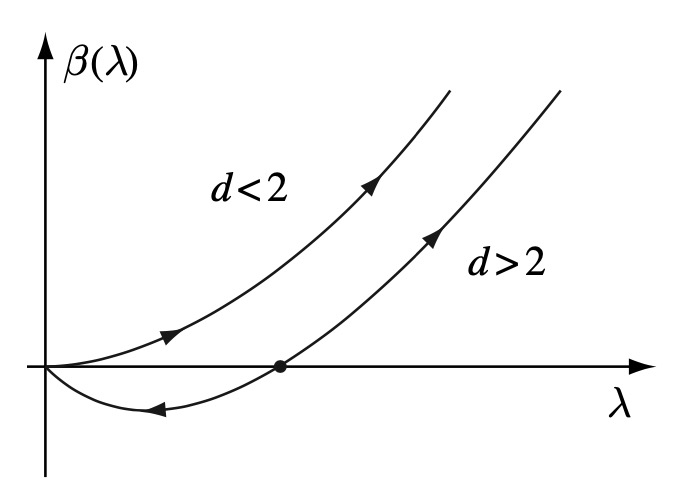
\includegraphics[width=0.3\linewidth]{pics/RG-flow.jpg}
\end{equation*}
From the beta function, we know at low dimension $d < 2$, $\beta(\lambda) > 0$.
In the low-energy limit, $1/\lambda \rightarrow 0$, i.e., the NL$\sigma$M would have little energy cost to create $\pi$ excitation.
The system is thus in the disordered phase.
On the other hand, for $d>0$, there is order-disorder transition at 
\begin{equation*}
	\lambda_* = \frac{4\pi(d-2)}{N-2}.
\end{equation*}
A special case is the O(2)-NL$\sigma$M at $d=2$, which requires additional analysis.



\section{BKT Phase Transition}

For the O(2) case, the NL$\sigma$M is described by an angle $\phi$:
\begin{equation}
	\mathcal L = \frac{1}{\lambda}(\partial_\mu\phi)^2 + g\cos(\phi),
\end{equation}
where we have introduced an external field for the later convenience.
We can renormalize $\theta$ so that the kinetic term is canonical:
\begin{equation}
	\mathcal L = \frac{1}{2}(\partial_\mu \phi)^2 + g\cos(\beta \phi),
\end{equation}
where $\beta=\sqrt{\lambda/2}$.
The external field term will be regarded as the perturbation, the running coupling $g$ will be computed by standard RG procedure.



\subsection{First Order Beta Function}
When write $\phi$ as the sum of slow and fast modes: $\phi=\phi_s+\phi_f$, the partition function is
\begin{equation}
	Z = \left\langle\exp\left\{-g \int d^2 x \cos\left[\beta(\phi_s+\phi_f)\right] \right\}\right\rangle_f \int D[\phi_s] \exp\left[-\frac{1}{2}\int d^2x (\partial_\mu\phi_s)^2\right].
\end{equation}
We then consider the effective action to the second order:
\begin{equation}
	S_{\mathrm{eff}} = S_0 + \langle S_1\rangle_f - \frac{1}{2}\langle S_1^2\rangle_f^c
\end{equation}
where $S_0$ comes from the kinetic term and $S_1$ the perturbation.
To the first order,\footnote{Note the identity: $\cos\left[\beta(\phi_s+\phi_f)\right]=\cos(\beta\phi_s)\cos(\beta\phi_f)-\sin(\beta\phi_s)\sin(\beta\phi_f)$. Note the fact that $\sin(\beta\phi_f)$ term will not contribute when integrated over the fast field.}
\begin{equation}
\begin{aligned}
	\langle S_1\rangle &= g \int d^2 x \left\langle\cos\left[\beta(\phi_s+\phi_f)\right] \right\rangle_f 
	= g \int d^2 x \cos(\beta\phi_s)\langle\cos(\beta\phi_f)\rangle_f.
\end{aligned}
\end{equation}
We then compute the expectation over the fast field:\footnote{Note that fact $\langle \exp(i\beta\phi_f)\rangle = \exp(-\frac{1}{2}\beta^2 \langle\phi_f^2\rangle)$.}
\begin{equation}
	\left\langle \cos(\beta\phi_f)\right\rangle_f
	= \left\langle \frac{e^{i\beta\phi_f} + e^{-i\beta\phi_f}}{2}\right\rangle_f
	= \exp\left({-\frac{1}{2}\beta^2\langle\phi_f^2\rangle}\right) 
	= \exp\left[-\frac{\beta^2}{4\pi}\int_{d\Lambda}\frac{dk}{k} \right] 
	= s^{-\beta^2/4\pi}.
\end{equation}
The coarse-graining $x\rightarrow x'=s^{-1}x$ produce additional $s^{2}$ factor
In this way, the rescaling of $g$ is:
\begin{equation}
	g \rightarrow s^{2-\frac{\beta^2}{4\pi}} g.
\end{equation}
Let $s=e^{dl}$, the beta in the first order is
\begin{equation}
	\frac{d \ln g}{dl} = 2-\frac{\beta^2}{4\pi}.
\end{equation}


\subsection{Second Order Field Renormalization}
Now consider the second-order expansion
\begin{equation}
	\langle S_1^2\rangle_f^c = \langle S_1^2\rangle_f - \langle S_1^2\rangle_f^2.
\end{equation}
The first term is (we denote $\phi(x_i)$ as $\phi_i$ for notational simplicity):
\begin{equation}
\begin{aligned}
	\langle S_1^2\rangle_f &= g^2 \int d^2x_1 d^2x_2 \langle \cos(\beta\phi_1) 
		\cos(\beta \phi_2) \rangle_f 
	= \frac{g^2}{2} \int d^2x_1 d^2x_2 \left\langle \cos\left[\beta(\phi_1+\phi_2)\right] + \cos\left[\beta(\phi_1-\phi_2)\right] \right\rangle_f \\
	&= \frac{g^2}{2} \int d^2x_1 d^2x_2 \left\{\langle\cos\left[\beta(\phi_{f,1}+\phi_{f,2})\right]\rangle_f\cos\left[\beta(\phi_{s,1}+\phi_{s,2})\right]  + 
	\langle\cos[\beta(\phi_{f,1}-\phi_{f,2})]\rangle_f\cos\left[\beta(\phi_{s,1}-\phi_{s,2})\right]\right\}.
\end{aligned}
\end{equation}
Similarly, we have neglect all $\sin(\beta\phi_f)$ terms.
The averaging gives:
\begin{equation}
\begin{aligned}
	\langle S_1^2\rangle_f
	= \frac{g^2}{2} \int d^2x_1 d^2x_2 \left\{e^{-\frac{\beta^2}{2}\langle[\phi_{f,1}+\phi_{f,2}]^2\rangle} \cos[\beta\phi_{s,1}+\beta\phi_{s,2}] + 
	  e^{-\frac{\beta^2}{2}\langle[\phi_{f,1}-\phi_{f,2}]^2\rangle} \cos[\beta\phi_{s,1}-\beta\phi_{s,2}] \right\}.
\end{aligned}
\end{equation}
For the second term,
\begin{equation}
\begin{aligned}
	\langle S_1\rangle_f^2 &= \left[g\int d^2 x \left\langle \cos(\beta\phi_s+\beta\phi_f)\right\rangle_f \right]^2 
	= \left[g\int d^2 x \cos(\beta\phi_s) \exp\left(-\frac{\beta^2}{2}\langle\phi_f^2\rangle_f \right)\right]^2 \\
	&= \frac{g^2}{2}e^{-\beta^2 \langle \phi_f^2\rangle_f} \int d^2x_2 d^2 x_2 \left\{ \cos[\beta(\phi_{s,1}+\phi_{s,2})] + \cos[\beta(\phi_{s,1}-\phi_{s,2})] \right\}
\end{aligned}
\end{equation}
The subtraction is
\begin{equation}
	S^{(2)}_{\mathrm{eff}}
	= g^2 e^{-\beta^2\langle\phi_f^2\rangle} \int_{x_1,x_2}  \left\{
		\left(e^{-\beta^2 \langle\phi_{f,1}\phi_{f,2}\rangle}-1 \right)\cos\left[\beta(\phi_{s,1} +\phi_{s,2})\right] 
	 + \left(e^{\beta^2 \langle\phi_{f,1})\phi_{f,x})\rangle}-1 \right)\cos\left[\beta(\phi_{s,1} -\phi_{s,2})\right] \right\}.
\end{equation}
Formally, the first term gives the correction to the external field, while the second term appears to be additional.
We will show in the following that the second term actually correct the kinetic term.
Consider the bosonic correlation
\begin{equation}
	\mathcal G(\bm x) \equiv \langle \phi_f(x) \phi_f(0)\rangle_f = F(\bm x) dl + O(dt^2).
\end{equation}
A straightforward calculation with the hard cut-off yields $F(\bm x)$ a Bessel function with long oscillating tail.
However, it can be shown that implementing a smooth cut-off will make $F(\bm x)$ short ranged.
For this reason, we can switch to the center-of-mass coordinate:
\begin{equation}
	\bm R = \frac{\bm x_1 + \bm x_2}{2}, \quad \bm r = \bm x_1 - \bm x_2.
\end{equation}
In this way, the term $\cos\left[\beta\phi_{s,1} +\beta\phi_{f,2}\right]$ is approximated by a $\cos\left[2\beta\phi_s(x)\right]$ term, which is oscillating at double frequency, and thus is regarded as irrelevant.

The remaining term can be simplified by the approximation:
\begin{equation}
	\cos\left[\beta\phi_{s,1} -\beta\phi_{s,2}\right]
	\sim 1-\frac{\beta^2}{2} [\bm r \cdot \nabla\phi_s(\bm R)]^2
\end{equation}
The constant term only contributes to the the infinity of free energy.
The non-trivial contribution is:\footnote{Note that fact: $\int d^2r\ r_i r_j = \delta_{ij} \int r dr d\theta\ r^2 \cos^2(\theta) = \pi \delta_{ij} \int dr\ r^3$.}
\begin{equation}
\begin{aligned}
	\int d^2 R \int d^2 r \left(e^{\beta^2 \langle\phi_{f,1}\phi_{f,2}\rangle}-1 \right)\cos\left[\beta\phi_{s,1} -\beta\phi_{s,2}\right] 
	&\simeq -\frac{\beta^4}{2} \int d^2 R \int d^2r F(\bm r) [\bm r \cdot \nabla\phi_s(\bm R)]^2 \\
	&\simeq -\frac{\pi \beta^4}{2} \left[\int_0^\infty dr\ r^3 F(r)\right]dl \int d^2 R [\nabla\phi_s(\bm R)]^2 \\
	&\equiv -\pi \beta^4 A dl \times \frac{1}{2}\int d^2 R [\nabla\phi(\bm R)]^2.
\end{aligned}
\end{equation}
We see the second order perturbation renormalize the free field, as it change normalization of the field:
\begin{equation}
	\phi \rightarrow \phi' = Z^{\frac{1}{2}} \phi, \quad 
	Z^{\frac{1}{2}} = 1 +\frac{g^2}{2} \pi \beta^4 A dl.
\end{equation}
To preserve the form of the $\cos(\beta\phi)$ term, we have to shift
\begin{equation}
	\beta \rightarrow \beta' = Z^{-\frac{1}{2}}\beta = \beta-\frac{1}{2}\pi g^2\beta^5 A dl.
\end{equation}
The RG-flow for $\beta$ is then
\begin{equation}
	\frac{d\beta}{dl} = -\frac{1}{2}\pi g^2\beta^5 A.
\end{equation}
Near the critical point 
\begin{equation}
	g_* = 0, \quad \beta_* = \sqrt{8\pi},
\end{equation}
we keep only lowest order term, the prefactor $e^{-\beta^2\langle\phi_f^2\rangle}$ is then neglected, and we will not consider second order correction to external field here.
We introduce a new set of variables:
\begin{equation}
	x \equiv 2 - \frac{\beta^2}{4\pi}, \quad
	y \equiv 4\pi \sqrt{8\pi A} g.
\end{equation}
The RG-flow is then
\begin{equation}
	\frac{dx}{dl} = y^2, \quad
	\frac{dy}{dl} = xy.
\end{equation}
The flow diagram is
\begin{equation*}
	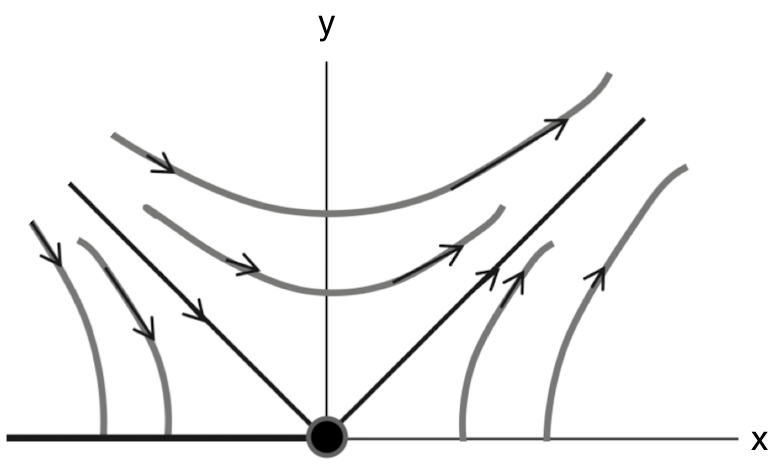
\includegraphics[width=0.3\linewidth]{pics/KT-RG-flow.png}
\end{equation*}
When $x+y<0$, the coupling will flow to $g=0$, corresponding to the KT phase; otherwise the coupling flows to $g\rightarrow\infty$ corresponding to the disordered phase.


\end{document}


